\documentclass[10pt]{article}
\usepackage{amsmath}
\usepackage{amssymb}
\usepackage{tikz}
\usetikzlibrary{shapes.geometric,arrows.meta,positioning, shapes.misc}
\usetikzlibrary{overlay-beamer-styles,positioning,decorations.pathreplacing,calligraphy}
\usetikzlibrary{hobby,shapes.misc}
\usetikzlibrary{positioning}
\usetikzlibrary{bayesnet}
\usepackage{color}
\usepackage{xcolor}
\usepackage[colorlinks=true, 
            citecolor = blue,
            linkcolor = black,
            pagebackref]{hyperref}

\newcommand{\argdot}{{\,\vcenter{\hbox{\tiny$\bullet$}}\,}}

\newcommand{\mc}{\mathcal}

\newcommand{\bb}{\mathbb}

\begin{document}

  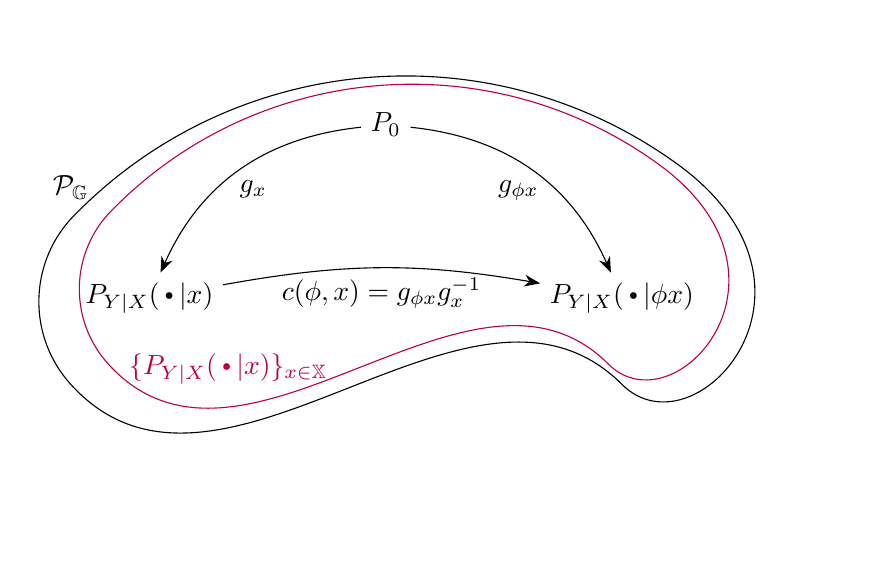
\begin{tikzpicture}[use Hobby shortcut]
    \node (A) at (1, -1) {$P_{Y|X}(\argdot|x)$};
    \node (B) at (7,-1) {$P_{Y|X}(\argdot|\phi x)$};
    \node (C) at (4,1.2) {$P_0$};
    \node (D) at (0,0.4) {$\mc P_{\bb G}$};
    \node (D) at (2,-1.9) {${\color{purple}\{P_{Y|X}(\argdot|x)\}_{x \in \bb X}}$};
\draw[rotate=-90,scale=0.7] (0,0) .. +(3,0) .. +(3,10) .. +(3,10) .. +(-1,11) .. (0,0); 
\draw[rotate=-90,scale=0.635,color = purple] (-0.1,0.75) .. +(3,0) .. +(3,10) .. +(3,10) .. +(-1,11) .. (-0.1,0.75); 
\draw[-{Stealth[length=2mm]}] (C) to [bend right=30] node [midway,below]{$\quad g_x$} (A) ;
\draw[-{Stealth[length=2mm]}] (C) to [bend left=30] node [midway,below]{$g_{\phi x}\quad$} (B) ;
\draw[-{Stealth[length=2mm]}] (A) to [bend left=10] node [midway,below]{${c(\phi,x) = g_{\phi x}g_x^{-1}}$} (B) ;
\end{tikzpicture}

\end{document}